\documentclass[12pt,a4paper]{scrartcl}

\title{Seatbelt Reminder System}
\subtitle{A small-scale embedded project using state machine approach}
\author{lkmuk}
\date{{\small started from 2020-07-10  \raggedleft  \\ last modified on \today \raggedleft \\}}

% typesetting arts
\usepackage[margin=2cm]{geometry}
\pagestyle{headings}
%\usepackage{fancyhdr}
%	\pagestyle{fancy}
%	\fancyhead{} %clear defaults
%	\fancyhead[L]{Developing a Seatbelt Reminder System}
%	\fancyhead[R]{\markleft}
%	\fancyfoot{} % clear defaults
%	\fancyfoot[C]{Page \thepage}
%	\fancyfoot[R]{version: \today}

\usepackage[bf,pagestyles,raggedright]{titlesec}
\titleformat{\section}
  {{\titlerule[0.8pt]}\vspace{3pt}{\titlerule[0.8pt]}\vspace{1em}\sffamily\Large\bfseries}
  {\thesection}
  {1em}{}
  []

\usepackage[yyyymmdd]{datetime}
	\renewcommand{\dateseparator}{-}
\usepackage{fontenc}
	\usepackage{palatino}
	

\usepackage{amsmath,amssymb}	
\usepackage[hidelinks]{hyperref}

%\usepackage{footnote}
%\makesavenoteenv{tabular}
%\makesavenoteenv{table}

\usepackage{array,float}

\usepackage{circuitikz}
\usepackage{siunitx}
\usepackage{tikz}
\usetikzlibrary{arrows,positioning,shapes.multipart}
\usepackage{standalone} %for schematics.tex

\newcommand{\umlState}[3]{
	\textbf{#1} 
	\nodepart{two}
	\small entry/{\ttfamily#2}\\
	exit/{\ttfamily#3}
}

\usepackage[style=numeric,backend=biber]{biblatex}
\addbibresource{doc-ref.bib}
% counters
%\setcounter{tocdepth}{2}
%\setcounter{secnumdepth}{3}
\newcommand{\readme}{\href{../readme.md}{\textit{readme} file}}



\usepackage[theorems,breakable]{tcolorbox}
\newtcbtheorem{prob}{Problem}{%
	colback=green!10, colframe=	green!10!black, fonttitle=\bfseries,
}{p}
\newtcbtheorem{notes}{Important Notes to the Implementation}{%
	colback=yellow!10, colframe=	orange!40!black, fonttitle=\bfseries,
}{notes}
\newtcbtheorem{tips}{Tips / Reminder}{
	colback=blue!10, colframe=	blue!70!black, fonttitle=\bfseries,
}{tips}
\newtcolorbox{codeline}[1]{
	colback=blue!10, colframe=	blue!70!black, fonttitle=\bfseries,
	title=#1,
	fontupper=\ttfamily,
	% select monospace font for contents
	fontlower=\rmfamily \small,
	breakable
}

\usepackage{color}
\definecolor{mygreen}{rgb}{0,0.6,0}
\definecolor{mygray}{rgb}{0.5,0.5,0.5}
\definecolor{mymauve}{rgb}{0.58,0,0.82}

\usepackage{listings}
\lstset{ 
	backgroundcolor=\color{white},   % choose the background color; you must add \usepackage{color} or \usepackage{xcolor}; should come as last argument
	basicstyle=\footnotesize\ttfamily,        % the size of the fonts that are used for the code
	breakatwhitespace=false,         % sets if automatic breaks should only happen at whitespace
	breaklines=true,                 % sets automatic line breaking
	captionpos=b,                    % sets the caption-position to bottom
	commentstyle=\color{mygreen},    % comment style
	deletekeywords={...},            % if you want to delete keywords from the given language
	escapeinside={\%*}{*)},          % if you want to add LaTeX within your code
	extendedchars=true,              % lets you use non-ASCII characters; for 8-bits encodings only, does not work with UTF-8
	firstnumber=1,                % start line enumeration with line 1000
	frame=single,	                   % adds a frame around the code
	keepspaces=true,                 % keeps spaces in text, useful for keeping indentation of code (possibly needs columns=flexible)
	keywordstyle=\color{blue},       % keyword style
	morekeywords={*,...},            % if you want to add more keywords to the set
	numbers=left,                    % where to put the line-numbers; possible values are (none, left, right)
	numbersep=5pt,                   % how far the line-numbers are from the code
	numberstyle=\tiny\color{mygray}, % the style that is used for the line-numbers
	rulecolor=\color{black},         % if not set, the frame-color may be changed on line-breaks within not-black text (e.g. comments (green here))
	showspaces=false,                % show spaces everywhere adding particular underscores; it overrides 'showstringspaces'
	showstringspaces=false,          % underline spaces within strings only
	showtabs=false,                  % show tabs within strings adding particular underscores
	stepnumber=5,                    % the step between two line-numbers. If it's 1, each line will be numbered
	stringstyle=\color{mymauve},     % string literal style
	tabsize=2,	                   % sets default tabsize to 2 spaces
	title=\lstname                   % show the filename of files included with \lstinputlisting; also try caption instead of title
}





\begin{document}
	\maketitle
	\begin{abstract}
		This documentation discusses the use of state machine approach in embedded development, in particular the state machine modeling framework and its implementation in C. 
		This is exemplified and demonstrated by the Seatbelt Reminder System prototype discussed in \cite{Wolf}. 
		The contributions here are 
		some modifications to the original solution and 
		supplementing that pseudo-C code with a full working prototype system.
		The problem description and development settings for this project can be found in \readme~and are generally not reproduced in this documentation.
	\end{abstract}
{\tableofcontents}

	

\section{High-level event-based modeling of the system {behavior} using state chart} \label{sec:UML_Statechart}
	This section discusses how to model the desired behavior of our Seatbelt Reminder System (as described in \readme) in an intuitive state chart\footnote{The transition precedence or \textit{sequence} mentioned in \S \ref{sec:state:transition:precedence} is not specified in the UML standard but it is widely adopted since it exploits the sequential execution nature of the implementation.}. 
	In the next section (\S \ref{sec:FSM_in_C}), we will convert the UML state chart \textit{``back to''} the classic FSM for our particular target setup 
	which can then be readily implemented in C.
	
	Before that, let's underline the major differences between UML state  chart and the conventional Finite State Machine (FSM) where the later was employed in \cite{Wolf}.
	
	\paragraph{state chart vs FSM}
	UML state chart provides substantial enhancements to FSM that ultimately lead to much simpler more manageable state machine model.\footnote{The price we pay is some framework support and/ or some additional (compile time) conversion to the classic FSM format, either manually or automatically.
	The conversion concept is addressed in \S \ref{sec:FSM_in_C}.}
	Below are some examples of the extensions:
	\begin{itemize}
		\item the notion of \textit{entry action}, 
			\textit{exit action}, or \textit{during action} of a state \\
			(the advantages of \textit{exit} and \textit{entry} action will be elaborated in \S \ref{sec:UML:during_entry_exit})
		\item notion of events for triggering state transitions.
			For our example, I decided to simply update the system periodically so the default event is \textit{an} ISR arrival.
			Another event will be timeout event for not fastening the seatbelt in time. Events will be part of the subject of \S \ref{sec:UML:transition:spec}.
		\item hierarchical and/or concurrent state behavior 
			which are integral to tackling the \textit{state explosion} issue for complex reactive systems and improving modularity, hence reusability (some discussion on that in \S \ref{sec:concurrent})
	\end{itemize}
		
	Of course, our standalone seatbelt reminder system by no means qualifies as a complex system so this section will not attempt to cover the concept of state composition with hierarchy and concurrency.
	Yet, the first two concepts are quite relevant for our example and therefore applied.
	Consequently, the state machine model given at the end of this section (Fig. \ref{fig:myUMLStateMC}) looks slightly different (to be precise, clearer) than the (finite) state machine presented in \cite{Wolf}.
	
	
	\subsection{Identifying system I/O} \label{sec:UML:IO}
		The FSM model in \cite{Wolf} has the following three inputs and output:
		{\color{gray} \small \itshape
		\begin{itemize}
			\item a sensor that detects whether a person sits on the seat,
			\item a sensor that detects whether the person has fastened his/her seatbelt,
			\item a timer input and
			\item a buzzer output.
		\end{itemize}}
		Since the FSM has to be executed or \textit{updated} regularly anyway, possibly at fixed (nominal) rate (with some acceptable jitter), we can simply infer the elasped time from sitting without fastening the seatbelt using the tricks presented in the following subsection 
		(\S \ref{sec:UML:list_states_n_counter_var}),
		thereby dispensing the timer input.\footnote{In fact, the aforementioned temporal logic of state charts assumes certain (in-system) support for timing behavior! }
	
		Moreover, for the demo, I prefer a simple red led to a buzzer. All these lead to the following \textbf{revised \textit{system} I/O specification}, as illustrated in Fig \ref{fig:pin_connection}.
		
		\begin{itemize}
			\item seat occupancy sensor (one might use this for other tasks...)
			\item seatbelt sensor
			\item red LED as a warning signal to the occupant and/ or driver.
		\end{itemize}

	\subsection{Enumerating states \& extended state variable(s)} \label{sec:UML:list_states_n_counter_var}
	Perhaps, one of the most critical aspect of employing state-machine based programming paradigms is the enumeration of some meaningful states. In many case, to prevent \textit{state explosion}, we might additionally \textit{extend} the qualitative nature of the state with some internal (quantitative) state variable(s). This comes at the cost of more complicated testing and can become less intuitive to interpret the state chart. 
	In many cases we might also have concurrent states which will not cover here.
	
	Fortunately with temporal event notion and the simplistic nature of our system, we \textit{can} specify the behavior entirely based on a qualitative finite set of states where each state is sufficient to capture previous system operation history.
	They are:
	\begin{description}
		\item [\texttt{IDLE}:] the initial state when there is simply no one sitting on the seat.
		\item [\texttt{SEAT\textunderscore NO\textunderscore BELT}:]	when the seat \textit{starts} to be occupied but the seatbelt is still not on.
		\item [\texttt{SEAT\textunderscore WITH\textunderscore BELT}:]	when both the seat is occupied and the seat belt is on.
		\item [\texttt{WARNING}:] when the seat is occupied for ``too long'' (say exceeding 6 consecutive seconds) without the seatbelt fastened.
	\end{description}
	
	
	
	\subsection{Identify possible state transitions} \label{sec:UML:reachbility}
	This step concerns simply the question 
	\textbf{\emph{whether it is possible}} to transit 
	from one state to another state.	
	From our previous discussion, our state machine has four states, so we can simply examine the possibility of all $4^2 - 4 = 12$ cases (excluding self-transition because self-transition will not be of interest until \S \ref{sec:UML:transition:spec}). 	
	An initial analysis of our Seatbelt Reminder System yields the one-step reachability table (Table \ref{tab:OneStepTransition}).
	
	\begin{table}[ht]
		\centering
		\caption{One-step reachability between states for our Seatbelt Reminder System}
		\begin{tabular}{|c||c|c|c|c|} \hline
			$\downarrow$ current state \textbackslash \ next state $\rightarrow$ 
			& 0 & 1 & 2 & 3\\ \hline
			0 (IDLE) & - & y & (y) & \\
			1 (SEAT\_NO\_BELT) & {\color{red}y} & - & y & y\\
			2 (SEAT\_WITH\_BELT) & (y) & y & - & \\
			3 (WARNING) & y & & y & -\\ \hline
		\end{tabular}
		\label{tab:OneStepTransition}
		
		
		\vspace{1em}
		\begin{tabular}{p{1cm} p{10cm}}
			where & 
		 ``y" denotes a very plausible one-step transition; 
		 \newline 
		``(y)'' denotes a \textit{Just-in-case}$\dagger$ backup transition; 
		\newline
		blank entries correspond to \textit{absolutely} impossible or unreasonable one-step transitions. 		\\
		& 
		\textit{$\dagger$ JIC in the sense that it might defy common sense (assuming integrity of the input data), e.g. leaving seat before releasing seatbelt as in one-step state transition: 2 to 0}
		\end{tabular}	
	\end{table}

	
	One might be tempted to skip this step and directly consider \textbf{\emph{how or under what conditions}} a state will transit to another (which is the step described in \S \ref{sec:UML:transition:spec}.	
	From my experience, it is \textit{better} not to skip this binary one-step reachability check.
	As a side note, the textbook solution omits or misses one of the transitions ({\color{red} from state 1 to 0}) which under certain scenario can lead to unexpected behavior --- longer time allowance for buckling up before triggering a warning signal.
			
	\subsection{Identify state transition actions}	\label{sec:UML:during_entry_exit}
		In many case, a state can be \textit{characterized} by what need(s) to be done as the (sub)system 
		leaves from this state (regardless of next state) or 
		enters into this state (regardless of previous state).
		These use cases lead naturally to the notion of \textit{exit} and \textit{entry actions} respectively. 
		This notion allows us to \textbf{avoid repetition} for the said use cases, hence \textbf{improved maintainability} \cite{Samek}. 
		
		Our example turns out to fit into this category of use cases very well. Indeed, we can model all transition actions in our case as either entry or exit actions!
	
		\subparagraph{Entry and exit action for state \textit{WARNING}} It is obvious that we should turn ON the warning lamp as we enter the \textit{WARNING} state
		whereas we should turn it OFF as we leave from it.
		
		\subparagraph{Entry action for state \textit{SEAT\_NO\_BELT}???} We might consider start of timing as an entry action but this is actually unnecessary \textit{at this stage}. We can leverage on the notion of timing events to emphasize what behavior we actually want, instead of implying how to implement this timing behavior.\footnote{Possible implementation schemes are HW counter (i.e. HW), or SW counter. The later is exploited here because of the rather tolerant timing requirements in our case and the simplicity. \label{fn:Implementation:Timer}}
	 
	\subsection{Specify transition conditions \& priorities} \label{sec:UML:transition:spec}
	\subsubsection{Events and Guards}
	In UML state chart notation, a state transition \textit{can}\footnote{see \S \ref{sec:state:transition:precedence} for the reason why it is not an adamant ``will''.} only take place when the corresponding \textit{event (class)} is triggered and the \textit{guard condition(s)} are meet. On a state chart, these information is encoded by the following syntax:
	\begin{center}
		Event name [the condition(s)] / state transition action(s); 
	\end{center}
	Note that a event in state chart needs not be a clock event. 
	A meaningful update event for a transition to be taken can really be anything, say when the \textit{seat sensor} registers a rising edge. 
	Whenever an event is missing on a transition arch, it just means ANY event can trigger such transition.
	Similarly, the guard condition is optional.
	
	
	\subsubsection{Temporal Logic} \label{sec:UML:TemporalLogic}
		In our example, the timing event of primary interest is the timeout event that \textit{should} trigger a warning signal:
		The trigger of state transition from \texttt{SEAT\textunderscore NO\textunderscore BELT}
		to \texttt{SEAT\textunderscore WITH\textunderscore BELT} can be modeled as \texttt{after($\alpha$ sec)}
		which says if the system is ``stuck'' at state \texttt{SEAT\textunderscore NO\textunderscore BELT}
		for $\alpha$ second transit to state \texttt{SEAT\textunderscore WITH\textunderscore BELT}.
		
		For the sack of completeness, it is worthwhile to note that one should refrain from modeling state chart with self-looping typical of many FSM \textit{implementations} because this is simply unnecessary\footnote{use \textit{during} actions instead} for the modeling stage and can lead to abstruse state machine model\footnote{If the self-loop is taken, it is deemed as leaving and \textbf{re}-entering that state, i.e. not counted as ``stuck'' at this state!}.
	\subsubsection{Exploiting the sequential execution nature}
	 \label{sec:state:transition:precedence}
	 A FSM at any given state MUST have \textbf{ONE deterministic} state transition, be it self-looping or transition to any other state.
	 Consequently, one always has to ensure each state has a set of exit transition (including self-looping) that covers the entire set of possible scenarios for each state. In the worst case, assuming we have $n$ binary inputs and no extended state variables, there are $2^n$ possible scenarios for each state. 
	 Furthermore, we will very likely end up with ``Spaghetti code'' --- fraught with if-else constructs and/or AND, OR operations to be evaluated as inside the if-condition test.
	 
	 Fortunately, state charts (geared towards sequential execution) permit us to considerably simplify the matter:
	
	\paragraph{Default transition} If there is no events that can trigger a transition, it is not unreasonable to deem the (sub)system to remain at this state. Note that this is NOT self-looping.
	
	Consequently, we are relieved from checking if \textit{each} state in the system has a ``complete'' set of transition conditions.
	\paragraph{Execution sequence or priority} Mainstream computers invariably execute code sequentially. As far as the execution of the update code (here, we assume there is only one for a state machine) is concerned, whether several transitions are triggered at the same time is irrelevant because \textbf{once} a (the first) valid trigger is found, \textbf{that} transition is taken.
	
	As a result, any transition from a given state does NOT have to be mutually exclusive which helps eliminating spaghetti coding. 
	Since this implies the possibility that multiple state transition triggers become valid at the same time, 
	we can simply assert the execution order or priority of the outgoing arches for each state to ensure \textit{determinism}.
	In fact, this might corresponds what we might intuitively have in mind!
	For our example, given the system is at state \texttt{SEAT\textunderscore NO\textunderscore BELT}
	which from previous discussion (Table \ref{tab:OneStepTransition}) has three possible transitions,
	it is logical to assign the highest priority to the transition to state \texttt{WARNING},
	i.e. we wish to start timing with minimal latency.
	The same argument applies if the system is at state	\texttt{SEAT\textunderscore WITH\textunderscore BELT}
	so we prioritize the transition to state \texttt{SEAT\textunderscore NO\textunderscore BELT}.
	
	Although it is not always straight forward to rank the relative importance, I decided to assign the priorities to all states that have multiple possible transitions.
	By doing so, we might on the one hand compromise some design freedom. On the other hand, such loss is minute or even non-existent if the transition conditions do not overlap.
	Above all, it is just a matter of \textit{who} decides it, either you or the tool. Furthermore, it is very straight forward to modify those priorities at a later point of time, shall there be such need.

	\subsection{The outcome of this stage: the state chart model}
	The principles outlined above yield the following visual formalism which can be served as the formal requirements specification of our Seatbelt Reminder System. 
	It is remarkable that such an intuitive graphical representation is actually expressive enough to capture all of the desired behavior.
	\begin{figure}[H]
		\centering
		\documentclass[12pt]{standalone}
\usepackage{tikz}
\usepackage{fontenc}
\usetikzlibrary{arrows, shapes.multipart, positioning}

\newcommand{\umlState}[3]{
	\textbf{#1} 
	\nodepart{two}
	\small entry/{\ttfamily#2}\\
	exit/{\ttfamily#3}
}

\begin{document}
	
	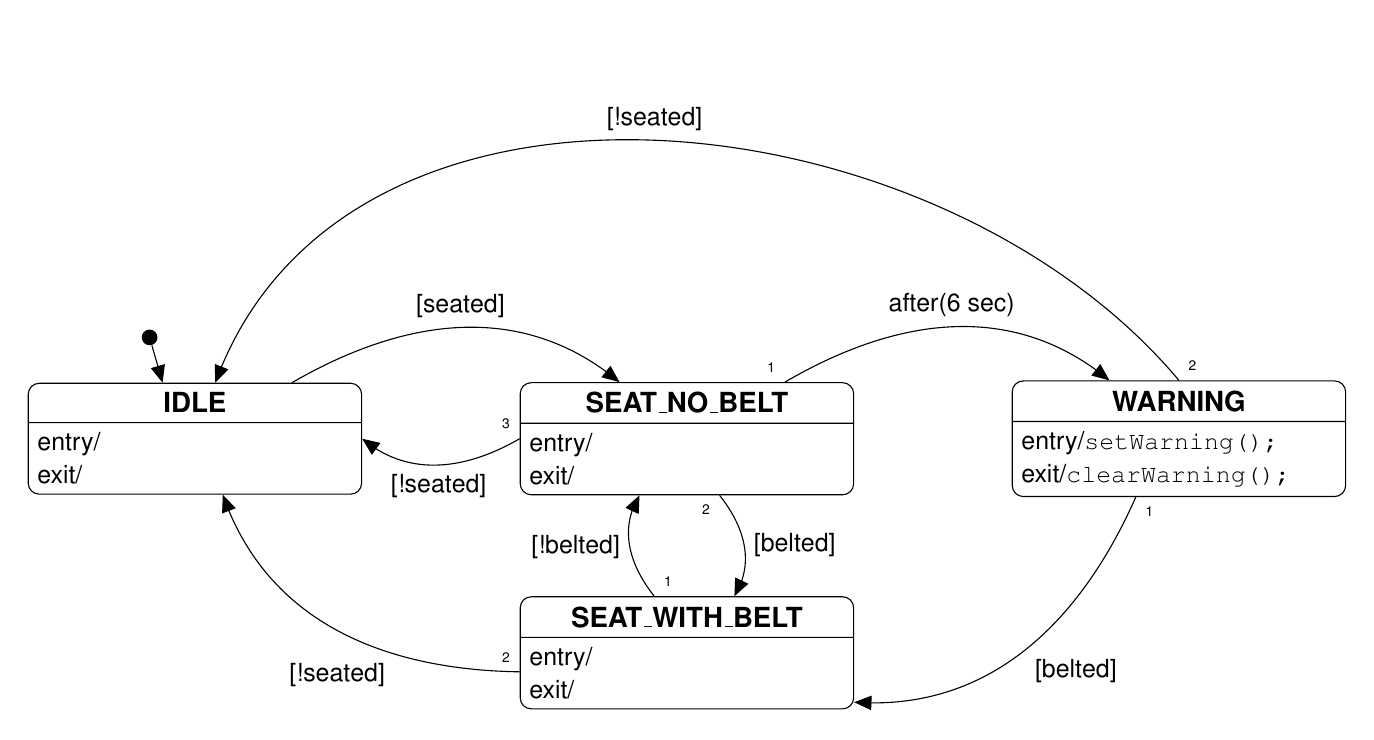
\begin{tikzpicture} %
		[
			font={\sffamily},
			every text node part/.style={align=center}, % sleeky thing behind nodeparts...
			state/.style={
				anchor=center,
				draw,
				rectangle split,
				rectangle split parts=2, 
				rectangle split part align={center, flushed left},
				rounded corners=4,
				minimum width=4.2 cm,%text centered,
				text width= 4 cm,
				node distance= 2 cm,
			},
			arch/.style={-triangle 45},
			transit/.style={font={\small \sffamily},midway},
			active/.style={red},
			stdBend/.style={bend left, in =140},
			priority/.style={font={\tiny \sffamily}},
		]
		\node[state] 
		(s0) {\umlState{IDLE}{}{}};
		\node[state, right =of s0] 
		(s1) 
		{\umlState{SEAT\textunderscore NO\textunderscore BELT}{}{}};
		\node[state, below =of s1.center] 
		(s2) 
		{\umlState{SEAT\textunderscore WITH\textunderscore BELT}{}{}};
		\node[state, right =of s1] 
		(s3)
		{\umlState{WARNING}
			{setWarning();}
			{clearWarning();}
		};
		\node[circle,inner sep=0, minimum size=2mm, fill=black](init)[above left =5mm and 5mm of s0.north]{};
		\draw[arch] (init) -- (s0.120);
		\draw[arch] 
		(s0) 
		to [stdBend] node[transit,above]{[seated]} 
		(s1);
		\draw[arch] 
		(s1) 
		to [stdBend] node[transit,above]{after(6 sec)}  node [pos=0,above left,priority]{1}
		(s3);
		\draw[arch] 
		(s1) 
		to [stdBend] node[transit,right]{[belted]} node [pos=0,below left,priority]{2}
		(s2);
		\draw[arch] 
		(s2) 
		to [stdBend] node[transit,left]{[!belted]} node [pos=0,above right,priority]{1}
		(s1);
		\draw[arch] 
		(s1.west) 
		to [stdBend] node[transit,below]{[!seated]} node [pos=0,above left,priority]{3}
		(s0.east);
		\draw[arch] 
		(s2) 
		to [stdBend] node[transit,below = 3mm]{[!seated]} node [pos=0,above left,priority]{2}
		(s0);
		% would this happen?...
		\draw[arch]
		(s3)
		to [stdBend] node[transit,below right]{[belted]} 
		node [pos=0,below right,priority]{1}
		(s2);
		\draw[arch]
		(s3.north)
		to [out = 130, in = 70] node[transit,above]{[!seated]} 
		node [pos=0,above right,priority]{2}
		(s0);
	\end{tikzpicture}	
\end{document}
		\caption{The resultant state chart of the Seatbelt Reminder System}
		\label{fig:myUMLStateMC}
	\end{figure}
	

\section{Implementing the state machine in C} \label{sec:FSM_in_C}
	Implementing the state machine as depicted by the state chart of Fig. \ref{fig:myUMLStateMC} often require some transformation into a conventional FSM which can be readily converted into a C-implementation.
	
	This transformation augments the state chart with more implementation specifications. In our example, these design specifications are mainly:
	\begin{itemize}
		\item A periodic polling implementation, i.e. the system gathers the input values at regular time interval of 0.5 ms, and updates the output according to the control logic;
		\item An additional software counter that track the elapsed time being at state \texttt{SEAT\textunderscore NO\textunderscore BELT}.
		Note that this approach exploits the 0.5-ms periodic occurrence of the update event. If this update event is aperiodic, we might need to resort to an independent HW counter (i.e. timer). 
		In fact, this counter regardless of how it is implemented becomes an extended state variable. 
		Its initialization and update will inevitably creates more transition actions.
		Furthermore, we have to convert the 6-sec allowance into appropriate threshold values to which the counter value compares.
	\end{itemize}
	
	The transformation also includes cascading state \textit{entry} and \textit{exit} actions into the relevant transition arches.
	The end result is summarized by an implementation specific FSM in \S \ref{sec:FSM:done}.
	
	\subsection{Implementing Temporal logic with SW counter}
		\paragraph{Implementing the 0.5 ms update cycle} \label{clk_tree}
			For the target hardware I used, the simplest way to implement the periodically updated FSM is via the \textit{SysTick Handler} in which the update code is written into the SysTick Interrupt Service Routine (ISR).
			
			The target clock tree is configured in such a way that the SysTick Interrupt Request (IRQ) arrives every 0.5 ms with acceptable precision. Fig \ref{fig:clock} shows part of the details which ultimately decides the SysTick timer input frequency.			
			\begin{figure}[ht]
				\centering
				\includegraphics[width=0.9 \textwidth]{clock-tree.png}
				\caption{The clock tree configuration used in this project. \newline
					The corresponding code is attached in \S \ref{app:startup}.}
				\label{fig:clock}
			\end{figure}
		
			The rest lies on the calculation of the required auto reload value for triggering a SysTick IRQ. 
			This can be calculated by $0.5~\text{ms} \times 4~\text{MHz} -1 = 1999$. 
			Note that the CMSIS \texttt{SysTick\textunderscore Config} function used in the code (see the \texttt{main} function in \ref{app:src_code:app}) does us a favor: 
			the ugly ``minus 1'' due to the fact the timer counts from 0 is abstracted away.
			
		\paragraph{The SW counter and additional transition actions}
			The following implementation decisions are made
			\begin{itemize}
				\item The counter is initialized as 1 every time the system enters state \texttt{SEAT\textunderscore NO\textunderscore BELT}.
				Note that it is advantageous to classify this as an entry action.
				\item Moreover, the counter is increment by 1 every time the system re-loops into this state.
			\end{itemize}
		\paragraph{The implementation-specific transition condition}
			Since the threshold for triggering a transition from state \texttt{SEAT\textunderscore NO\textunderscore BELT}
			to \texttt{WARNING} should \textit{correspond} to the duration of 
			$$\frac{6~ \text{sec}}{0.5~\text{ms per update events}} = 12000~\text{update events}. 		$$	
			With the counter initialization and update actions defined as above, the threshold value should also be 12000.
			In our implementation, this is simply to replace the \textit{after(6 sec)} in Fig.~\ref{fig:myUMLStateMC}
			with a conventional condition:
			\hfill
				[counter \textgreater 12000]
			\hfill.\footnote{As mentioned earlier, it can be a bit tricky to inspect the counters: the corresponding threshold actually depends on how or when we initialize them, how they are incremented/ decremented as well as whether you use \textgreater ~comparison or $\geq$.}
	
	\subsection{Cascading the transition actions} \label{sec:FSM:cascade}
		Now, it is the right time to cascade all
		the elegant \textit{entry} and \textit{exit} actions
		into a single transition action for each transition arch.
		
		For our case (a non-hierarchical state machine), 
		the cascading involves 3 parts:
		
		Suppose the system is leaving from state X into state Y in which this transition has an additional transition action. 
		The cascading is as simple as just combining these actions in the following order:
		\begin{enumerate}
			\item exit action of state X, followed by...
			\item (arch-specific) transition action from state X to Y, and then
			\item entry action of state Y.
		\end{enumerate}
	
	\subsection{The resultant FSM} \label{sec:FSM:done}
	\begin{figure}[H]
		\centering
		\documentclass{standalone}
\usepackage{tikz}
\usepackage{fontenc}
\usetikzlibrary{arrows, shapes.multipart, positioning,automata}


\begin{document}
	
	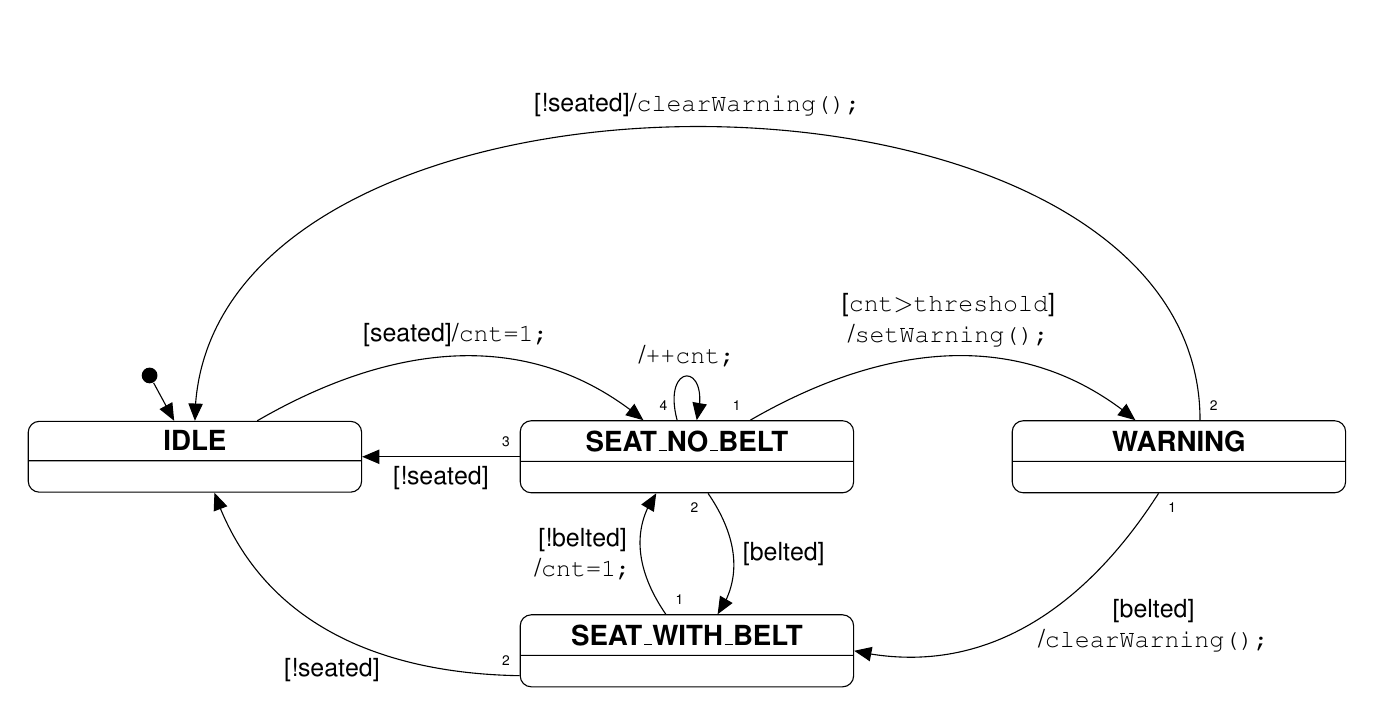
\begin{tikzpicture} %
		[
			font={\sffamily},
			every text node part/.style={align=center}, % sleeky thing behind nodeparts...
			state/.style={
				anchor=center,
				draw,
				rectangle split,
				rectangle split parts=2, 
				rectangle split part align={center, flushed left},
				rounded corners=4,
				minimum width=4.2 cm,%text centered,
				text width= 4 cm,
				node distance= 2 cm,
			},
			arch/.style={-triangle 45},
			transit/.style={font={\small \sffamily},midway},
			active/.style={red},
			stdBend/.style={bend left, in =140},
			priority/.style={font={\tiny \sffamily}},
		]
		\node[state] (s0) {\textbf{IDLE}};
		\node[state, right =of s0] (s1) {\textbf{SEAT\textunderscore NO\textunderscore BELT}};
		\node[state, below =of s1.center] (s2) {\textbf{SEAT\textunderscore WITH\textunderscore BELT}};
		\node[state, right =of s1] (s3)
		{\textbf{WARNING}};
		\node[circle,inner sep=0, minimum size=2mm, fill=black](init)[above left =5mm and 5mm of s0.north]{};
		
		\draw[arch] (init) -- (s0.120);
		
		\draw[arch] (s0) 
			to [stdBend] node[transit,above]{[seated]/\texttt{cnt=1;}} 
			(s1);
		\draw[arch] 
			(s1) 
			to [stdBend] node[transit,above]{[\texttt{cnt\textgreater threshold}]\\/\texttt{setWarning();}}  node [pos=0,above left,priority]{1}
			(s3);
		\draw[arch] 
			(s1) 
			to [loop above] node[transit,above]{/\texttt{++cnt;}}  
			node [pos=0,above left,priority]{4}
			(s1);
		\draw[arch] 
		(s1) 
		to [stdBend] node[transit,right]{[belted]} node [pos=0,below left,priority]{2}
		(s2);
		\draw[arch] 
		(s2) 
		to [stdBend] node[transit,left]{[!belted]\\/\texttt{cnt=1;}} node [pos=0,above right,priority]{1}
		(s1);
		\draw[arch] 
		(s1.west) 
		-- node[transit,below]{[!seated]} node [pos=0,above left,priority]{3}
		(s0.east);
		\draw[arch] 
		(s2) 
		to [stdBend] node[transit,below = 2mm]{[!seated]} node [pos=0,above left,priority]{2}
		(s0);
		% would this happen?...
		\draw[arch]
		(s3)
		to [stdBend] node[transit,right]{[belted]\\/\texttt{clearWarning();}} 
		node [pos=0,below right,priority]{1}
		(s2.east);
		\draw[arch]
		(s3.60)
		to [out = 90, in = 90] node[transit,above]{[!seated]/\texttt{clearWarning();}} 
		node [pos=0,above right,priority]{2}
		(s0);
	\end{tikzpicture}	
\end{document}
		\caption{The resultant FSM of the Seatbelt Reminder System. 
			Apparently, it is more implementation oriented and less intuitive than Fig. \ref{fig:myUMLStateMC} 
			because of both the cascading of state actions and the extended state variable. 
			In this implementation, the extended state variable is \texttt{cnt}. 
			To \textit{correctly} implement the specified behavior in Fig. \ref{fig:myUMLStateMC}, 
			it is not only necessary to convert the 6-sec into the appropriate \texttt{threshold}, 
			but also to calculate the proper initial value!}
		\label{fig:myFSM}
	\end{figure}

	\subsection{Update the state value} 
	Actually, the cascading in \S \ref{sec:FSM:cascade} misses a critical part:
	\textit{updating the system state} 
	so that in the next update cycle 
	the system is on the ``right track'' to decide where to transit to.
	It is appropriate to \textit{integrate} the cascading steps above with 
	a memory update --- overwriting the (global) state variable.
	
	To minimize \textbf{latency in updating our output} (which is ideally the first action of the cascaded transition action sequence), it is advantageous to execute the state update last --- i.e. \textit{appending} the cascading steps.
	
	Therefore, the cascading in any implementation indeed looks like:
	\begin{enumerate}
		\item exit action of state X, followed by...
		\item (arch-specific) transition action from state X to Y, and then
		\item entry action of state Y, and finally
		\item update the state variable (named \texttt{stateSeat1} in my code).
	\end{enumerate}

	\subsection{The resultant C-code Implementation}
	The FSM in Fig. \ref{fig:myFSM} can be 
	\textbf{easily and efficiently} implemented using a \textit{switch}-construct
	as follows:
	
	\begin{codeline}{Snippet of the ISR implementing the FSM in Fig. \ref{fig:myFSM} written in C}
		\lstinputlisting[language=C]{fsm-c.txt}
		\tcblower
		The complete application source file (with more inline comments, variable declarations and overhead of polling input values) is attached in \ref{app:src_code:app}.
		The notation in the code is more verbose compared to Fig. \ref{fig:myFSM}.
		The correspondences should be clear.
	\end{codeline}

	We might replace all the \texttt{break;} keyword with \texttt{return;} 
	to further reduce program size and the runtime. 
	This is possible here because the SysTick ISR 
	has no other code to execute after this FSM.

%	\subsection{More details}
%		\paragraph{\texttt{enum} typedef instead of preprocessing \texttt{define}-directive} for obvious reasons.
%			Encoding of state, manual value assignment???
%		\paragraph{Initialization} of state variable and internal variables (if necessary) as \textit{static} variables that ideally only modified by one process, in my case, the SysTick handler process.
%	
%		\paragraph{Optimal permutation of case blocks?} The C-switch construct in \S \ref{sec:FSM:done} might lead to the impression that we might be able to minimize some reaction latency metric by exploring various permutations of case-blocks. In our example, there are $4!=24$ possible permutations.
%		
%		Anyhow, the disassembly of the corresponding object file which is slightly more indicative of performance suggests the actual execution order is conceptually divided into three parts:
%		\begin{enumerate}
%			\item An overhead of fetching the current state \& compare it with all cases in the same? order as the C-switch construct.
%			\item then the instructions for the corresponding state (corresponding to the C-statements for the current state \textit{case})
%			\item jump to the remaining tasks of the ISR
%		\end{enumerate}
%	
%		This means 
%		
%		* less comparison overhead? self-modifying code??? cache
%		
%		* the length of the correponding segment has no bearing!
%		
%		* keeping your ISR or thread program short as key!		
%		
%		For our small project without any other competing interrupts or any strict timing requirements, this advanced topic is provided more for completeness.
		
		
		
		
%		the invariably sequential nature of the FSM implementation in which 
%		the ISR process keeps comparing the current state with the immediate operands one-by-one (state-by-state) until it finds the right case (state) and jump to the corresponding code segment (corresponding to the C-statements inside that case block) and finally exits.
%		
%		This gives rise to the freedom to arrange the case blocks. There are in total $4! = 24$ possible permutations for our example. The effect of advanced cache and branch prediction technologies\footnote{Branch prediction to the appropriate state segment should be straight forward and quite successful because the current state is dedicated by the previous invocation.}, as well as compiler optimization might be helpful for deciding the optimal permutation but these will be out of the scope of this project.
%		
%		Instead, I decided that it is of highest priority to minimize the delay from sitting to start of timing (transition 0 to 1) so the segment for state 0 is scanned first in the execution.
%		and switching off the warning signal is least time-critical so state 3 last.
%		
%		These \textit{happen to} yield the same cardinal ordering of states.
%		
%		\paragraph{other optimization potential}
%			optimize the latency behavior by:
%			\begin{itemize}
%				\item ``optimal'' interrupt priority and preemption settings --- this involves system-wide optimization for complex system.
%				\item self-modifying code?! 
%			\end{itemize}
%		
%		
%		Instead, delay-criticality. Happens to be 0,1,2,3
		




\section{The bigger picture}
\subsection{Testing and Tool support} \label{sec:testing}
	\paragraph{Verification of the implementation}
	At this stage, we want to prove the \textit{correctness} of our implementation \textbf{with respect to the state chart model}. 
	I plan to post a video to show some black-box test cases.
	
	\paragraph{Validation of the state chart}
	This project is all about prototype demonstration (i.e. a hobby project). 
	We did not really systematically validate the model specification
	at the first place. What we did was pretty much thought experiments!
	If it turned out we had misunderstood the requirements, it would cost 
	some time to correct our implementation.
	
	\paragraph{Tool support}
		On top of that, the manual conversion from the state chart model to implementation code can be error-prone.
		
		Notwithstanding these shortcomings in our demo project, 
		the model-based programming (or cyber-physical system design, in general) approach \textit{can} actually streamline the entire development process.
		It allows us to validate our requirements as early as possible through \textit{simulation}
		while the model-to-implementation conversion process if automated (i.e. \textit{code generation}) \textit{can} ensure \textit{correct} implementation. 
		All we need are some sort of development tool support, possibly with some also some runtime support.
		
		In the future, I might also update this project to incorporate more tool support.
	
\subsection{Deploying concurrent state machines into a single target} \label{sec:concurrent}
	What if we want to deploy several \textit{instances} of the Seatbelt Reminder System into the same MCU?
	A conventional way is a \textit{superloop} that is more like round-robin scheduling but this scheduling is fixed at compile time. Obviously, this is not necessarily the most efficient way to handle such physical parallelism.
	
	With event-driven paradigm, we can \textit{model} each instance as a \textit{concurrent} state machine. Thereby, we can readily \textit{reuse} the artifacts in this project.
	\cite{Samek} provides great details regarding this aspect.

\section*{References}
\addcontentsline{toc}{section}{References}	
\printbibliography[heading=none]
\newpage
\appendix
	\section{Schematics of the System}
		Please check Figure \ref{fig:pin_connection}. You might also want to see \S \ref{sec:UML:IO} which defines the system input/ output.
		\begin{figure}[H]
			\centering
			\documentclass[11pt]{standalone}
\usepackage{tikz}
\usepackage{fontenc}
	\usepackage{palatino}
\usepackage[hidelinks]{hyperref}
\usetikzlibrary{positioning}
\usepackage{circuitikz}
\usepackage{siunitx}
\begin{document}
\begin{circuitikz}[font={\bfseries\fontfamily{qag}\selectfont}]
  \def \xSepBoardToConnector {3}
  \def \yLED {12cm}
  \node[
  	rectangle, minimum width = 8 cm, minimum height = 19 cm,
  	anchor = north east, fill=cyan!10,draw=black
  	] at (-\xSepBoardToConnector,6) (board) {};
	  \node[below = of board.north, 	text width = 10cm, align=center,] 
	  		{\huge Nucleo-F103RB\\ \normalsize Development Board};
  \node[
  	rectangle, draw, 
	  minimum width = 3cm, minimum height = 3cm,
  ] (MCU) at (board.center)  {MCU};
  
  \def \myPushPull(#1){
  	\draw (0,0) 
  	to ++(1,0)
  	to[R=220~\si{\ohm}] ++(0,2)
   	to[C=10 nF] ++(0,2)
   	to 	++(1,0)
   	to [push button={#1}]++(0,-4)
   	to[short,-o] (0,0);
   	
   \draw  (1.5,4) to[short,*-] ++(0,0.5) node[above] {3.3~V};
   \draw  (1,0) to[short,*-, R=5 k$\Omega$] ++(0,-2) node[ground]{};
   }
	  \myPushPull(SeatSensor)
	  \draw[-triangle 60](0,0) -- node[pos = 0, above left] {to MCU PA6} 
	  	++(-\xSepBoardToConnector,0) 
	  	--++(-1cm,0) |-(MCU.30);
  \begin{scope}[yshift=-8cm]
  	\myPushPull(BeltSensor)
  	\draw[-triangle 60](0,0) -- node[pos = 0, above left] {to MCU PA7} 
  	++(-\xSepBoardToConnector,0) 
  	--++(-1cm,0) |-(MCU.east);
  \end{scope}
	\draw
		(-\xSepBoardToConnector,-\yLED) to[R={330~\si{\ohm}},f_={\mbox{PA4}}]
		++(2.5,0) to [led,a={warning indicator}] 
		++(4.3,0) node[ground]{};		
	\draw [-triangle 60]
		(MCU.south) |- (-\xSepBoardToConnector,-\yLED);
	
	\node[
		circle, minimum size=1cm, draw=black,fill=white,
		above left = 1cm and 1cm of MCU.north, 
		label={\small HSE CLK @ 8 MHz}
	](HSE Clock) {};
	\draw (HSE Clock.center) -- ++(2mm,0);
	\draw (HSE Clock.center) -- ++(0,3mm);
			
	\draw[-triangle 60] (HSE Clock.east) -| (MCU.north);
	
\end{circuitikz}

	
	
\end{document}


			\caption{A schematics showing the pin assignment of the MCU and its external connections}
			\label{fig:pin_connection}
		\end{figure}
	
	\section{The source files}	
	\subsection{application C-code} \label{app:src_code:app}
		\lstinputlisting[language=C]{../app.c}
	\subsection{Startup file} \label{app:startup}
		The startup code and clock configuration function 
		were adapted from \cite{ASM} in which
		the clock configuration function is adapted according to the specifications in \S \ref{clk_tree}.
		
		\lstinputlisting[tabsize=4]{../startup.S}
		 
\end{document}

